\documentclass[9pt,a9paper,handout]{beamer}
\usepackage[T1]{fontenc}
\usepackage[utf8]{inputenc}
\usepackage[francais]{babel}
\usepackage{amsmath,amsfonts,amssymb,tikz,colortbl,lmodern,xspace,subfigure}
\usepackage{siunitx,array,url} % Symboles, etc
\usetheme{Berlin}
\usecolortheme{seagull}
\setbeamertemplate{caption}{\raggedright\insertcaption\par}
\setcounter{tocdepth}{1}

\defbeamertemplate*{footline}{myfootline} {
  \leavevmode%
  \hbox{%
      \begin{beamercolorbox}[wd=.32\paperwidth,ht=3ex,dp=1ex,left]{title in head/foot}%
        \scriptsize\hspace{4px}\insertshortauthor
      \end{beamercolorbox}%
      \hspace*{-5px}
      \begin{beamercolorbox}[wd=.34\paperwidth,ht=3ex,dp=1ex,center]{title in head/foot}%
%        \scriptsize\insertshortinstitute
      \end{beamercolorbox}%
      \hspace*{-5px}
      \begin{beamercolorbox}[wd=.36\paperwidth,ht=3ex,dp=1ex,right]{title in head/foot}%
        \scriptsize\insertshortdate{}\hspace*{2em}
        \scriptsize\insertframenumber{} / \inserttotalframenumber\hspace*{2ex} 
      \end{beamercolorbox}
  }%
  \vskip0pt%
}
\defbeamertemplate*{title page}{customized}[1][]
{
  \vbox{}
  \vfill
  \begingroup
    \centering
    \begin{beamercolorbox}[sep=8pt,center,#1]{title}
      \usebeamerfont{title}\inserttitle\par%
      \ifx\insertsubtitle\@empty%
      \else%
        \vskip0.25em%
        {\usebeamerfont{subtitle}\usebeamercolor[fg]{subtitle}\insertsubtitle\par}%
      \fi%     
    \end{beamercolorbox}%
    \vskip1em\par
    \begin{beamercolorbox}[sep=8pt,center,#1]{author}
      \usebeamerfont{author}\insertauthor
    \end{beamercolorbox}
    \begin{beamercolorbox}[sep=8pt,center,#1]{institute}
      \usebeamerfont{institute}\normalsize \insertinstitute
    \end{beamercolorbox}
    \begin{beamercolorbox}[sep=8pt,center,#1]{date}
      \usebeamerfont{date}\insertdate
    \end{beamercolorbox}\vskip0.5em
    {\usebeamercolor[fg]{titlegraphic}\inserttitlegraphic\par}
  \endgroup
  \vfill
}
\defbeamertemplate*{headline}{myheadline} {
    \begin{beamercolorbox}[colsep=1.5pt]{upper separation line head}
    \end{beamercolorbox}
    \begin{beamercolorbox}{section in head/foot}
    \vskip2pt\insertnavigation{\paperwidth}\vskip2pt
    \end{beamercolorbox}%
    \begin{beamercolorbox}[colsep=1.5pt]{lower separation line head}
    \end{beamercolorbox}
}


\makeatother
\setbeamertemplate{footline}[myfootline]

\title{Caractérisation de pointes fibrées dans l'optique d'une nano-pince optique plasmonique}
\author{Félix Piédallu}
\date{29 Juin 2016}
\institute{Grenoble INP Phelma, Filière Physique - Nanosciences\\Institut Néel - Équipe NanoOptique et Forces}

\begin{document}

\begin{frame}
    \maketitle
    \begin{center}
        \vspace*{6mm}
        
\includegraphics[width=50px]{Images/logo_phelma}
        \hspace*{4cm}
        
\includegraphics[width=50px]{Images/logo_neel}
        %
\includegraphics[width=40px]{Images/logo_cnrs}\qquad
        \\[0.2cm]
        Sous la direction de Jochen Fick
    \end{center}
\end{frame}


\section{Contexte du stage}
% Présentation de la pince optique
\begin{frame}
    \frametitle{Contexte du stage}
    
    \begin{columns}[T]
    \begin{column}{0.70\textwidth}
        {\large Les nanopinces optiques:}\\
    \quad Confinement de particules par gradient d'intensité lumineuse
    \begin{itemize}
        \item Faisceau focalisé (objectif de microscope): manipulations difficiles
        \vspace*{3mm}
        \item Faisceau collimaté (pointes fibrées): \\intégration et manipulations plus faciles
    \end{itemize}
    \vspace*{-5mm}
    \begin{figure}[H]
        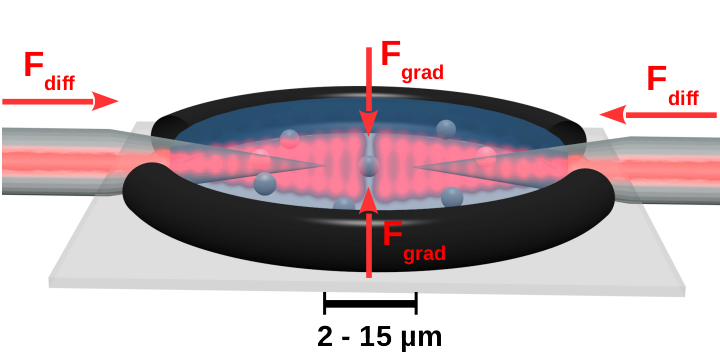
\includegraphics[width=0.7\textwidth]{Images/SchemaExperience.png}
    \end{figure}
    \end{column}
    \begin{column}{0.3\textwidth}
        \begin{figure}[H]
            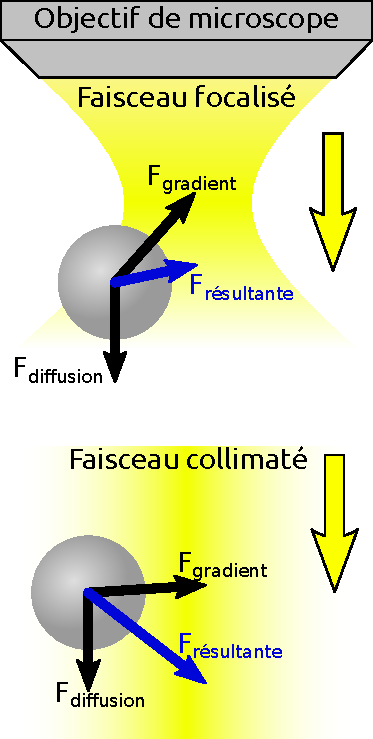
\includegraphics[width=0.82\textwidth]{Images/FaisceauConfinement.pdf}
        \end{figure}
    \end{column}
    \end{columns}


\vspace*{5mm}
    {\large $\rightarrow$ Caractérisation des pointes} \vspace*{1mm}\\
    \qquad Caractérisation spatiale et spectrale de l'émission


\end{frame}


\section{Élaboration des pointes}
\begin{frame}
    \frametitle{Élaboration des pointes fibrées}

    \vspace*{-4mm}
    \begin{columns}[c]
    \begin{column}{0.6\textwidth}
        {\large Gravure chimique en pointe}
        \vspace*{1mm}\\
        \qquad \qquad "Tube etching" au HF
    \end{column}
    \begin{column}{0.4\textwidth}
        \begin{figure}[H]
            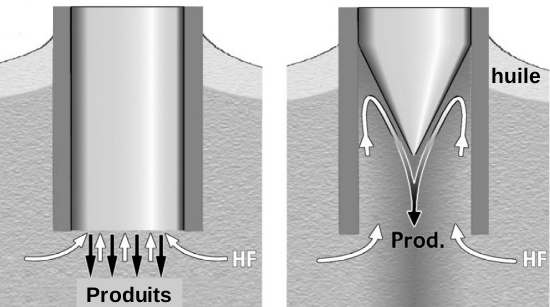
\includegraphics[width=\textwidth]{Images/gravure.png}
        \end{figure}
    \end{column}
    \end{columns}
    \vspace*{2mm}
    \begin{columns}[c]
    \begin{column}{0.6\textwidth}
        {\large Dépôt métallique et découpe au FIB}
        \vspace*{1mm}\\
%        "Tube etching" au HF
    \end{column}
    \begin{column}{0.4\textwidth}
        \begin{figure}[h]\centering
            \includegraphics[width=0.47\textwidth]{{"Images/l33fm2_avant_crop"}.jpg}
            \;
            \includegraphics[width=0.47\textwidth]{{"Images/l33fm2_apres_crop"}.jpg}
            \vspace{-3mm}\caption{Avant et après découpe FIB}
        \end{figure}
    \end{column}
    \end{columns}

\vspace*{2mm}
    \begin{figure}[h]\centering
        \includegraphics[width=0.47\textwidth]{{"Images/Pointe_metallique_air"}.jpg}
        \vspace{-3mm}\caption{Pointes métallisée et non métallisée}
    \end{figure}
    \let\thefootnote\relax\footnotetext{Jean-François Motte \& Gwenaëlle Julie, Institut Néel}
\end{frame}


\section{Émission spatiale des pointes}
\begin{frame}
    \frametitle{Émission spatiale des pointes}
    Scans en (y, z) de l'émission d'une pointe grâce à une autre pointe
    \begin{figure}[c]\centering
        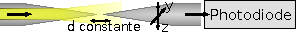
\includegraphics[width=0.6\textwidth]{Images/FibresScan.pdf}
    \end{figure}
    \vspace*{3mm}
    \begin{itemize}
        \item Mesure de l'angle d'émission des pointes non métallisées
        \begin{itemize}
            \item Dans l'air: 18\si{\degree}
            \item Dans l'eau: 8\si{\degree}
        \end{itemize}
    \end{itemize}
    \vspace*{-8mm}
    \begin{figure}[c]\centering\hspace*{35mm}
        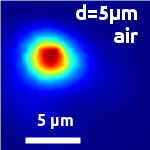
\includegraphics[height=0.15\textwidth]{Images/Spot_small.png}
        \quad
        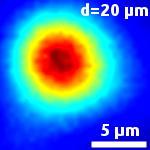
\includegraphics[height=0.15\textwidth]{Images/Spot_big.png}
        \quad
        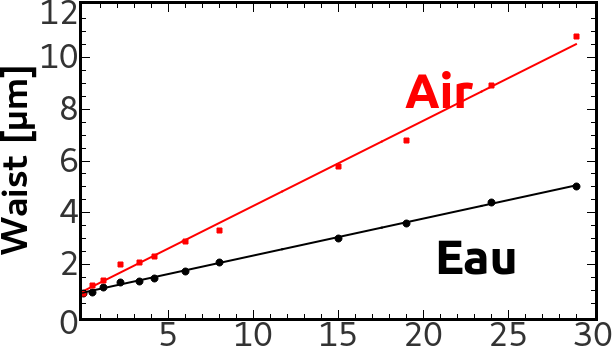
\includegraphics[height=0.15\textwidth]{Images/DistanceNues.png}
    \end{figure}
    
    \begin{itemize}
        \item Pointes métallisées
        \begin{itemize}
            \item Faible distance uniquement
            \item Diminution de l'excentricité avec la distance
            \item Forte dépendance en polarisation
        \end{itemize}
    \end{itemize}


    \begin{figure}[c]\centering
        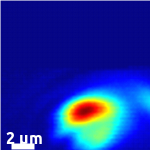
\includegraphics[height=0.13\textwidth]{Images/Metal_50nm.png}
        \quad
        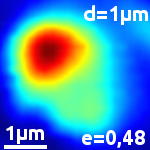
\includegraphics[height=0.13\textwidth]{Images/Metal_1um.png}
        \quad
        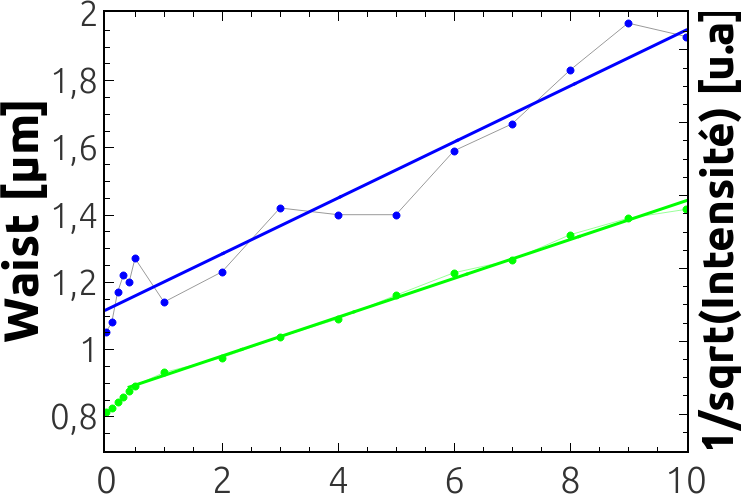
\includegraphics[height=0.18\textwidth]{Images/DistanceMetal.png}
        \qquad
        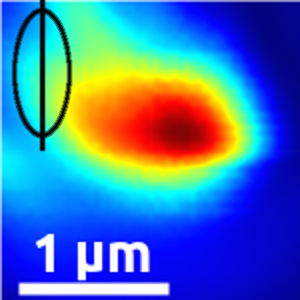
\includegraphics[height=0.13\textwidth]{Images/polar_long.png}
        \quad
        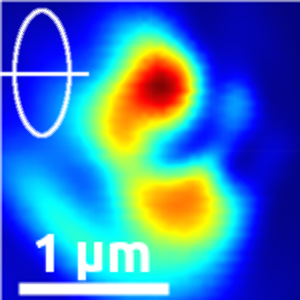
\includegraphics[height=0.13\textwidth]{Images/polar_trans.png}
    \end{figure}

\end{frame}


\begin{frame}    
    \frametitle{Émission spatiale des pointes de Bessel}
    {\large Pointe et faisceau de Bessel}%\footnote
    \vspace*{-2mm}\\
    \begin{figure}[H]
        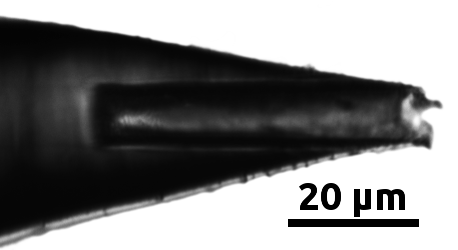
\includegraphics[width=0.20\textwidth]{Images/Bessel_1.png}
        \qquad
        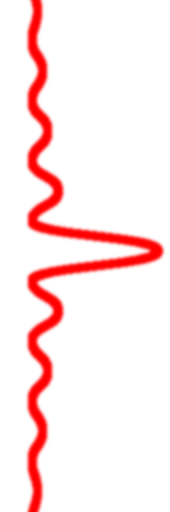
\includegraphics[width=0.40\textwidth]{Images/bessel.png}
    \end{figure}
\vspace*{0mm}

\vspace*{4mm}
    {\large Profil d'émission et évolution spatiale} \vspace*{1mm}\\
        \begin{figure}[t]\centering
        \vspace*{-3mm}
         \includegraphics[width=0.15\textwidth]{{"Images/bessel_profil"}.png}
            \;
            \includegraphics[width=0.35\textwidth]{{"Images/bessel_courbe"}.png}
            %\vspace{-3mm}\caption{Découpe au FIB}
        \end{figure}
        
    \begin{itemize}
        \item Grande distance de travail
        \item Faisceau "auto-réparant"
    \end{itemize}
    \let\thefootnote\relax\footnotetext{Samir R. Mondal, \textit{Central Scientific Instruments Organization} à Chandigarh (Inde)}
\end{frame}


\section{Émission spectrale des pointes}
\begin{frame}
    \frametitle{Émission spectrale des pointes}
    
    \begin{columns}[T]
    \begin{column}{0.60\textwidth}
        {\large Injection de lumière blanche}
        \begin{itemize}
            \item Spectres en transmission
            \begin{itemize}
                \item Pointe non métallisée
                \includegraphics[width=0.7\textwidth]{{"Images/Spectro_nue_nue"}.pdf}
                \item Pointe métallisée (ouverture $\varnothing \simeq 950nm$)
                \includegraphics[width=0.7\textwidth]{{"Images/Spectro_metal_nue"}.pdf}
            \end{itemize}
            \vspace*{1cm}
            \item Meilleure transmission dans l'eau
            \vspace*{1cm}
            \item Longueur d'onde de coupure pour les fibres métallisées
        \end{itemize}
    \end{column}
    \begin{column}{0.4\textwidth}\flushright
        \begin{figure}[h]
                \includegraphics[width=0.98\textwidth]{{"Images/Intensite_toutes"}.png}
        \end{figure}
        \begin{figure}[h]
                \includegraphics[width=\textwidth]{{"Images/Transmission_toutes"}.png}
        \end{figure}

    \end{column}
    \end{columns}

\end{frame}

\begin{frame}
    \frametitle{Conclusion}
    \begin{itemize}
        \item Pointes non métallisées utilisables en champ lointain
        \item Pointes de Bessel utilisables à très grande distance
        \item Couplage plasmonique dans les pointes métallisées en champ proche
    \end{itemize}
\end{frame}

\begin{frame}
    \begin{LARGE}
    \begin{center}
    \textbf{Merci de votre attention !}
    \vspace{0.5cm}
    
    \textbf{N'hésitez pas si vous avez des questions.}
    \end{center}
    \end{LARGE}
\end{frame}
\end{document}
